\section{Implementation}\label{sec:impl}
This project was implemented through MATLAB and carried out in two stages outlined below.
The encode stage takes in an image file and a watermark phrase and outputs a watermark embedded image.
The decode stage takes in a watermarked image and an original image and outputs the extracted watermark in text format.

\subsection{Encoding}
\begin{figure}[tbph]
  \centering
  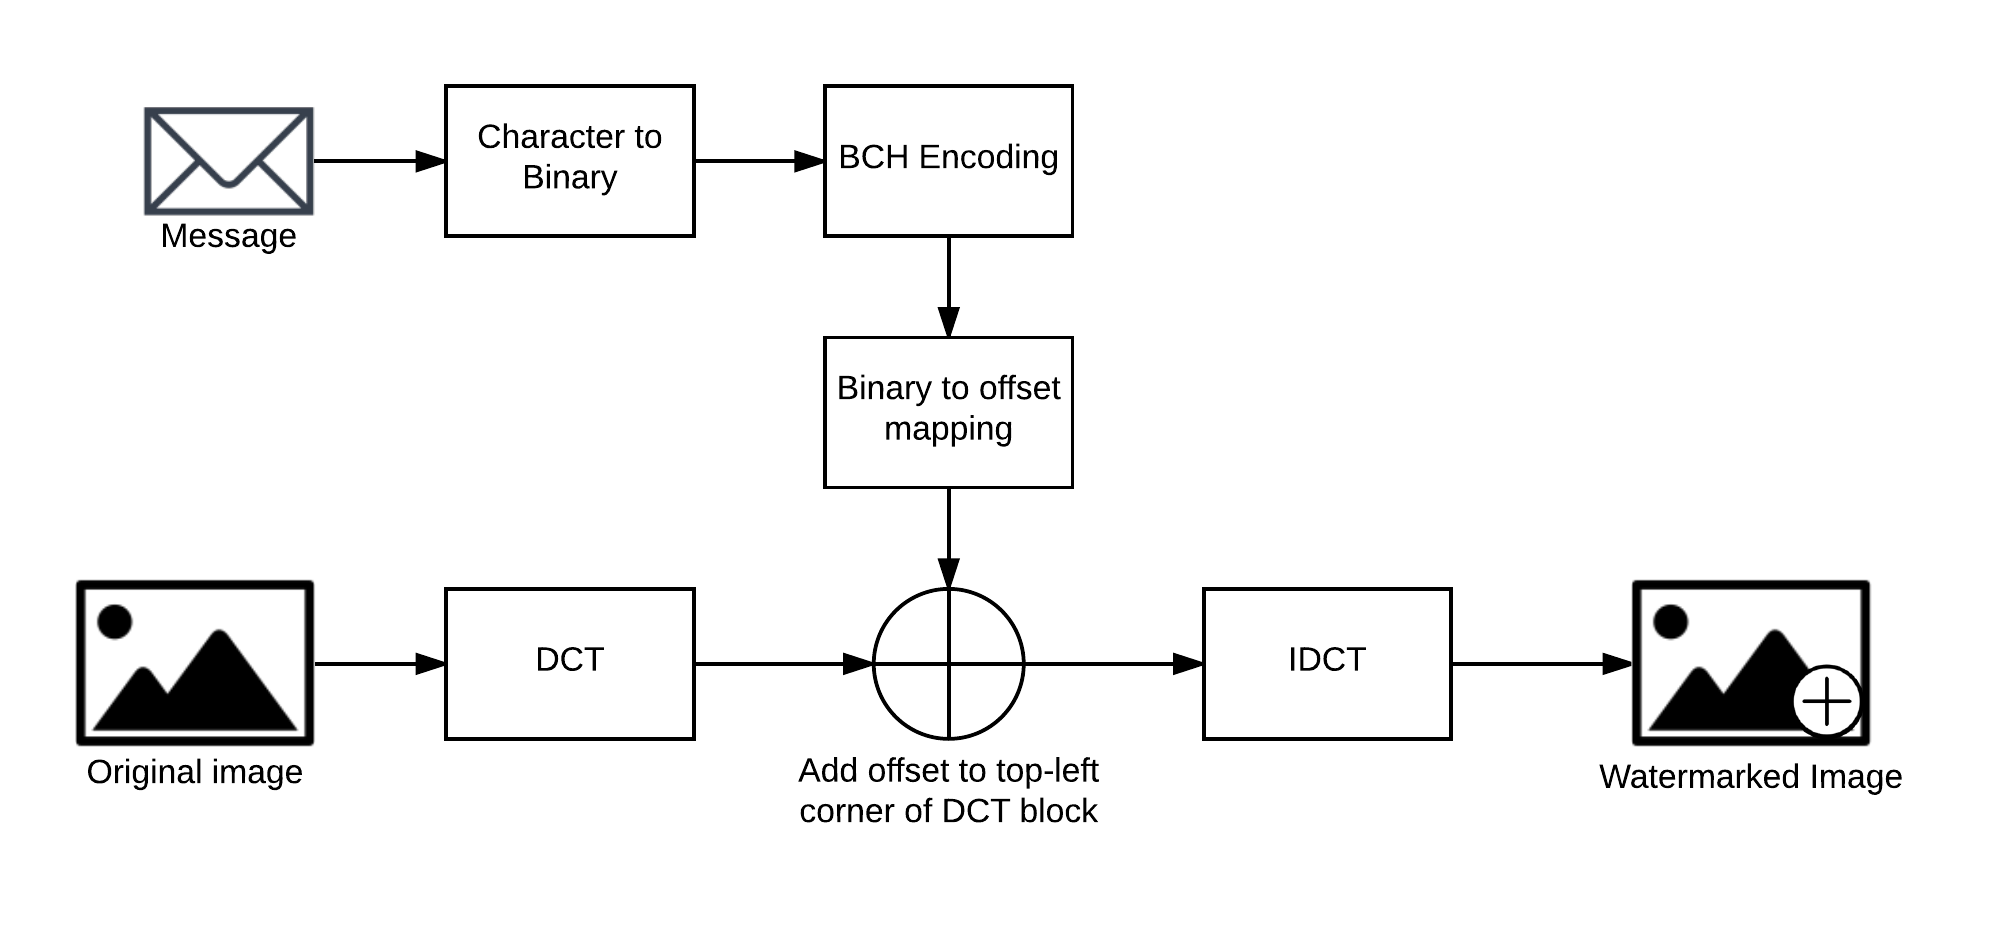
\includegraphics[width=0.75\linewidth]{graphics/encode}
  \caption{Watermark encoding process}
  \label{fig:encode}
\end{figure}

The watermark encoding function of this project is implemented through a MATLAB “m file”.
The file reads an image as input and also reads a string from the user as the watermark message.
The message must be in basic alphanumeric format and the length is limited to less than 33 characters.
This character limit is due to the requirements of the error correction methods, which will be discussed in the following sections.

The blockproc function is used to obtain the 8x8 DCT coefficients of the input image.
The watermark string is mapped letter by letter as a digit from 0 to 26, corresponding to its frequency in the english alphabet.
By employing this mapping method, we ensure that the most frequently used letters are mapped to the smallest numerical values.
The decimal values are converted to a base 6 binary format, and are then converted to a single long binary string.

In order to facilitate error correction, BCH coding was employed.
BCH coding takes a binary sequence and appends a binary correction code sequence to it.
This long binary string can be fed back into the BCH function, in the decoding stage, to produce an error-corrected binary sequence for our use in mapping back to the correct watermark message.

The binary sequence with the BCH correction code is then inserted into the top left corner of each of the DCT blocks of the image, bit by bit, as an offset.
By targeting those corners, the impact of the offsets on the quality of the overall image is minimized.
Once the watermark sequence is embedded, the image is inverse DCT and outputted to the user, ready for decoding.

\subsection{Decoding}
\begin{figure}[tbph]
  \centering
  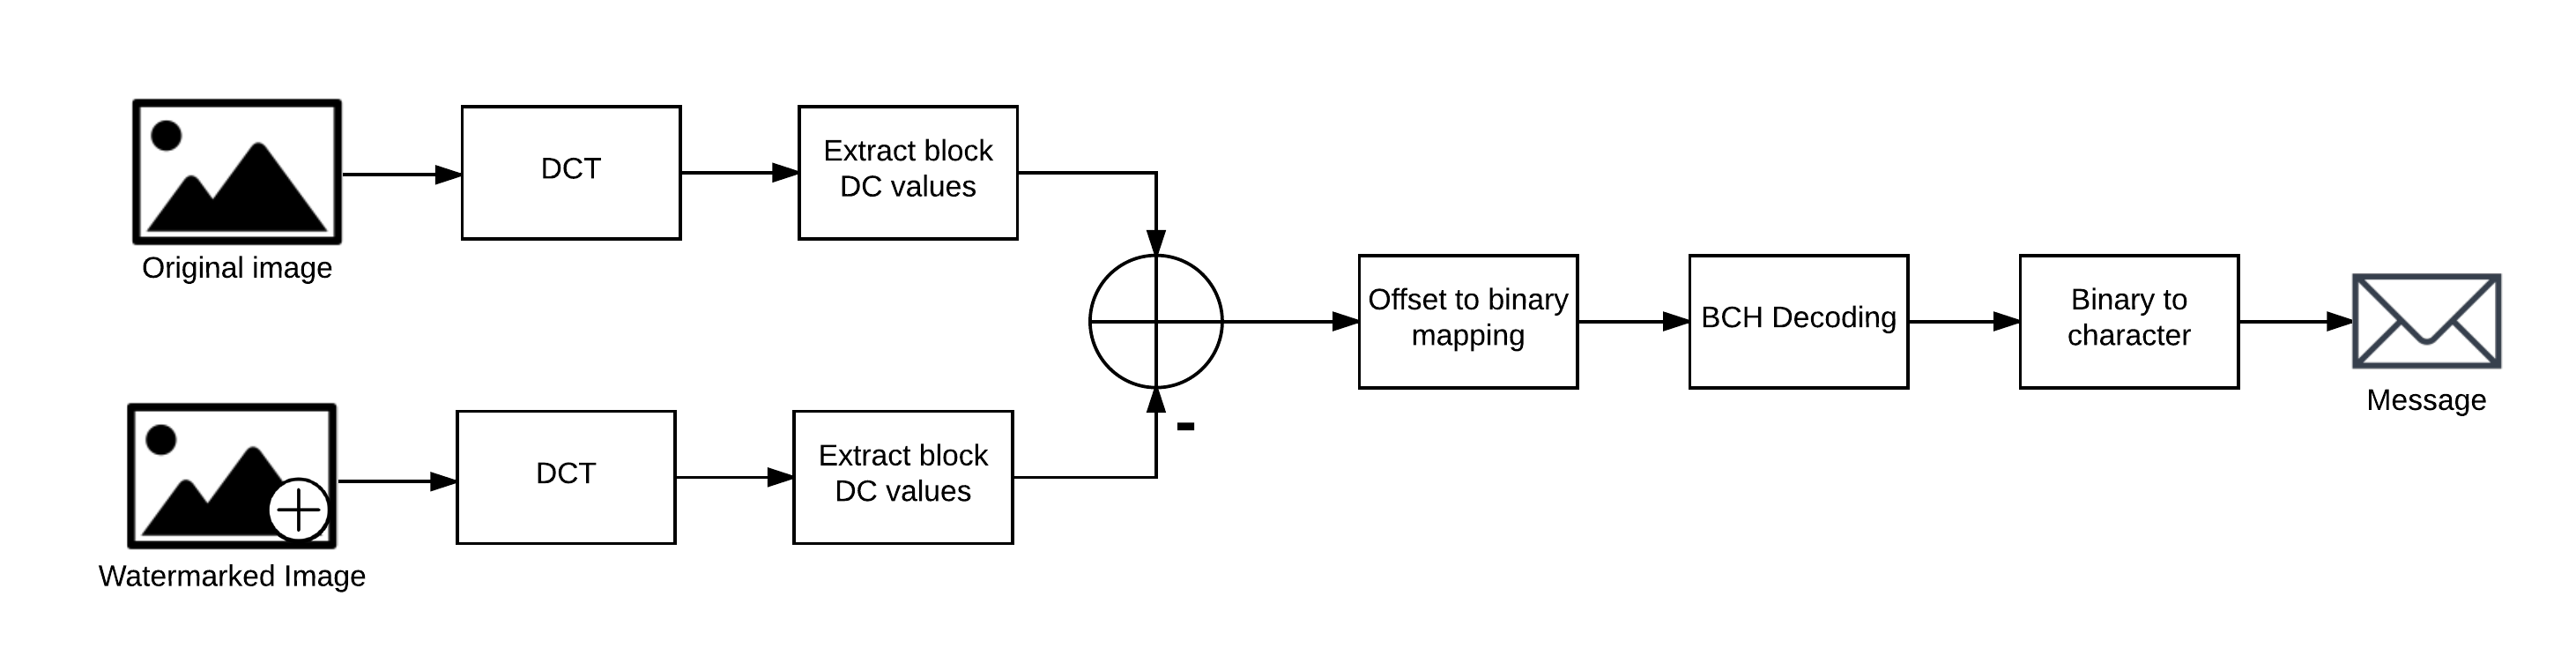
\includegraphics[width=0.95\linewidth]{graphics/decode}
  \caption{Watermark decoding process}
  \label{fig:decode}
\end{figure}

Similar to encoding, the decoding function of this project was also implemented through a MATLAB “m file”.
The file reads the watermarked image as an input, as well as the original, unwatermarked image.
The DCT coefficients of both images are acquired and the top left corner values of each block is compared to the corresponding value from the other image.
The difference is the offsets string.

This offsets string is then forced to a binary format, truncated to the correct length, and sent to through MATLAB’s BCH decoding function, where the correction code is employed in extracting the binary version of the original watermark message.
This binary code is run through an inverse mapping process and the final alphanumeric message is presented to the user as the extracted watermark.
